\chapter{Methodology}
\label{sec:methodology}

As discussed in Section \ref{sec:intro}, a two-step process is presented as a means of extracting knowledge from whole building electrical meters. Figure \ref{fig:framework} illustrates the intermediate steps in each of the phases.

The first step is to extract temporal features that produce quantitative data to describe various phenomenon occurring in the raw temporal data. This action is intended to transform the data into a more human-interpretable format and visualize the general patterns in the data. In this step, the data are extracted, cleaned, and processed with a library of temporal feature extraction techniques to differentiate various types of behavior. This library is outlined in Sections \ref{sec:statisticsfeatures}-\ref{sec:patternbasedfeatures}. These features are visualized using an aggregate heat map format that can be used evaluated according to expert intuition, comparison with design intent metrics, or with outlier detection. Section \ref{sec:temporalfeatureextraction} gives a more detailed definition of temporal features and how they're utilized in this study.

The second step is focused on the characterization of buildings using the temporal features according to several objectives. This step allows an analyst to understand the impact each feature has upon the discrimination of each objective. Five test objectives are implemented in this study: principal building use, performance class, operations strategy, general industry class, and energy savings measure success. One of the key outputs of this supervised learning process is the detection and discussion of what input features are \emph{most important} in predicting the various classes. This approach gives exploratory insight into what features are important in determining various characteristics of a particular building amongst a large set of its peers. These metadata are building blocks for many other techniques such as benchmarking, diagnostics and targeting. The motivation for choosing these particular objectives centers around the consistently available meta-data from the collected case study data and their relation to various other techniques in the building performance analysis domain. These topics are covered through qualitative discussion with several of the operations teams on the campuses where the data were collected and is discussed more thoroughly in Section \ref{sec:characterization}.

\begin{figure}[ht!]
\begin{center}
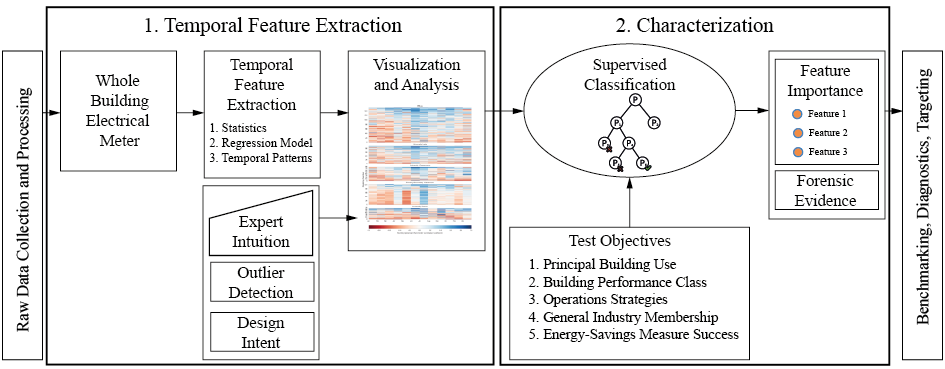
\includegraphics[width=1\columnwidth]{figures/process/FrameworkOverview3}
\caption{Overview of Data Screening Framework}
\label{fig:framework}%
}
\end{center}
\end{figure}


\section{Temporal Feature Extraction}
\label{sec:temporalfeatureextraction}

Feature extraction is an essential process of machine learning and is the means by which objects are described quantitatively in a way that algorithms can differentiate between different types or classes. Figure \ref{fig:convfeatures} illustrates a hierarchical node diagram of the features, or metadata, about a building that is often necessary to accumulate to perform conventional analysis from the literature. Much of these data are needed when creating an energy simulation model, when setting thresholds for automated fault detection and diagnostics, or benchmarking a building. When performing analysis on a single building, these meta-data might be easy to accumulate. However, when such a process is scaled across hundreds or potentially thousands of buildings, a collection of these data is not a trivial procedure. 
%This reality is reinforced through site interviews with campus-level energy managers as described later in this thesis.

%force chart data and viz in /Dropbox/04_ANALYSIS

\begin{figure}[ht!]
\begin{center}
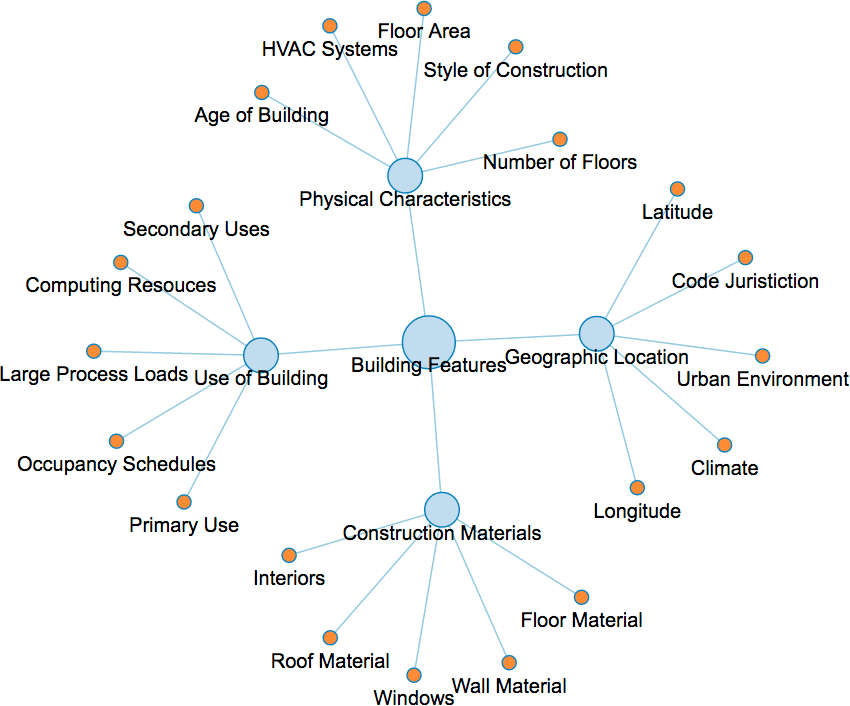
\includegraphics[width=0.7\columnwidth]{figures/TypicalFeatures/nontemporalforcechart}
\caption{Conventional features, or metadata, about a building
\label{fig:convfeatures}%
}
\end{center}
\end{figure}

Modern, whole building electrical meters measure and report raw, sub-hourly, time-stamped data. Significant amounts of essential information can be extracted from temporal data to characterize a commercial building. The harvest of this information can assist in the implementation of conventional analysis techniques, as inputs to classify or benchmark a building, or to predict whether a building is a good candidate for individual energy savings measures. To extract information solely from these sensors, new features can be created from these raw data. These features are designated as temporal as they summarize behavior occurring in time-series data. To illustrate the concept of temporal features qualitatively, Figure \ref{fig:electricalmeters_oneyear} shows four example hourly electrical meters from different buildings. Even to the untrained eye, these data streams show obvious differences in the way each building operates. Building A seems to be an extremely consistent consumer of energy across the entire year. There are no steady-state shifts in operation and seemingly no influence from outside factors. Qualitatively, this data stream can be thought of as \emph{consistent} or \emph{predictable}. Building B is similar in operation but has an obvious influence from an external factor in the summer months. It is safely assumed that the consumption of this building is weather-dependent, and it has some kind of cooling system. Building C illustrates behavior that has \emph{shifts} in consumption over the course of the year. This observation implies that this building has different schedules over the course of a year. Building D seems to have combinations of all of these attributes, with no obviously dominating phenomena. 


\begin{figure}[ht!]
\begin{center}
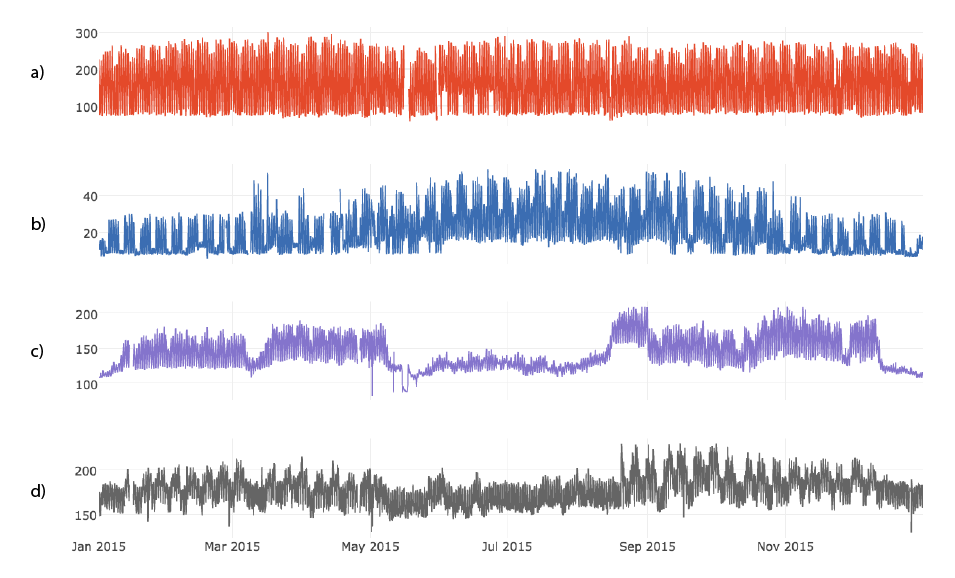
\includegraphics[width=0.98\columnwidth]{figures/temporal_metering_examples/temporal_metering_examples}
\caption{One year of example whole building electrical meter data that qualitatively exemplifying various temporal features
\label{fig:electricalmeters_oneyear}%
}
\end{center}
\end{figure}

Figure \ref{fig:electricalmeters_twoweeks} illustrates the same four buildings with the time range constrained to two weeks of data. Short-term temporal effects at the weekly and daily level are now observed. Building A still appears very consistent with a predictable daily cyclical pattern and a few variations around August 4 and 5. Building B exhibits similar behavior, but with noticeable weekend differences on Saturdays and Sundays. Building C has less observable daily patterns but has a trend upwards in the last five days of the time range. Building D, again, has a combination of these attributes.

\begin{figure}[ht!]
\begin{center}
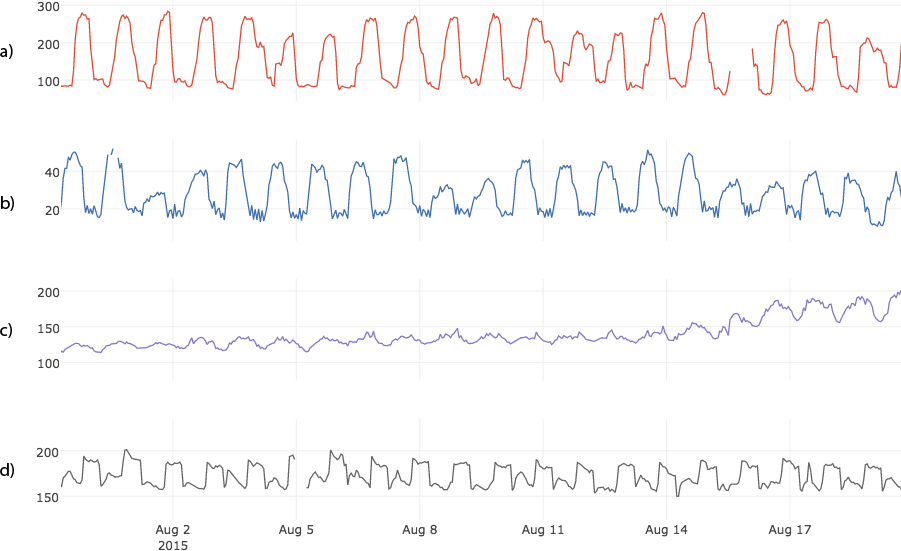
\includegraphics[width=0.98\columnwidth]{figures/temporal_metering_examples_zoomedin/temporal_metering_examples_zoomedin}
\caption{Two weeks of example whole building electrical meter data that qualitatively exemplifying various temporal features
\label{fig:electricalmeters_twoweeks}%
}
\end{center}
\end{figure}

The goal of temporal feature extraction and analysis is to use various techniques to convert all these \emph{qualitative} terms into a \emph{quantitative} domain. For example, the descriptor \emph{weather-dependency} can be quantified through the use of the Spearman rank order correlation coefficient with outdoor air temperature. Consistency or volatility of daily, weekly, or annual behavior can be quantified using various pattern recognition techniques. The primary focus of this study is to create and apply some temporal feature extraction techniques on commercial buildings for the purpose of characterization. Figure \ref{fig:temporalfeatures} illustrates the categories of temporal features created in this effort.

\begin{figure}[ht!]
\begin{center}
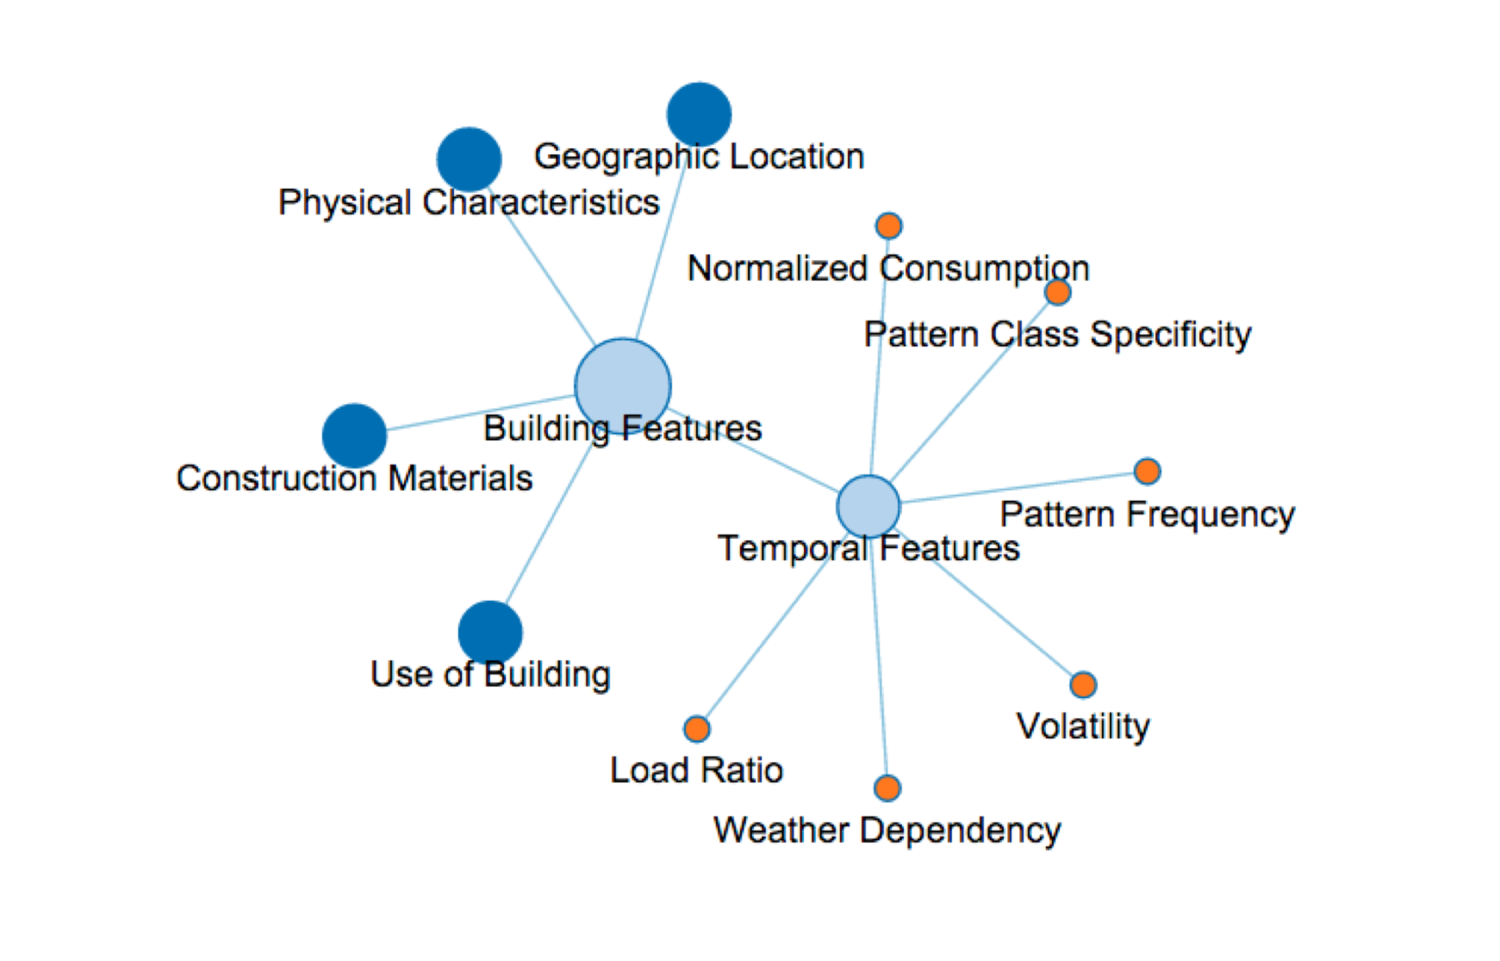
\includegraphics[width=0.7\columnwidth]{figures/TemporalFeatures/TemporalFeatures}
\caption{Temporal features extracted solely from raw sensor data
\label{fig:temporalfeatures}%
}
\end{center}
\end{figure}

Temporal features are aggregations of the behavior exhibited in time-series data. They are characteristics that summarize sensor data in a way to inform an analyst through visualization or to use as training data in a predictive classification or regression model. Feature extraction is a step in the process of machine learning and is a form of dimensionality reduction of data. This process seeks to quantify various qualitative behaviors. This section provides and overview of the categories of temporal features extracted from the case study building data, the methods used to implement them, and visualized examples of a selected subset of features manifest themselves over a time range. Table \ref{tab:featureoverview} gives an overview the temporal features outlined in this section.  A detailed list of the temporal features created in this Section can be found in Appendix A. 

\begin{table} 
    \begin{tabular}{| p{8cm} | p{6cm}  |}
        \textbf{Feature Category} &  \textbf{General Description}\\ 
        \hline
        Statistics-based & Aggregations of time series data using mean, median, max, min, standard deviation \\ 
        \hline
        Regression model-based & Development of a predictive model using training data and using model parameters and outputs to describe the data \\ 
        \hline
        Pattern-based &  Extraction of frequent and useful daily, weekly, monthly, or long-term patterns\\ 
        \hline
    \end{tabular} 
    \caption{Overview of feature categories}
\end{table}
\label{tab:featureoverview}

\section{Characterization and Variable Importance}
\label{sec:variableimportance}

The primary goal of this dissertation is to get a better sense of what behavior in time-series sensor data is most characteristic of various \emph{types} of buildings. As mentioned in the introduction, if this meta-data can be discriminated, the process of characterizing a building can be automated. In this section, the process of using random forest classification models and the input variable importance feature.

For each objective, several steps are taken to predict each objective and then to investigate the influence of the input features on class differentiation:
\begin{enumerate}
\item A random forest classification model is built using subsets of the generated features to predict the objectives class
\item The classification model provides an indication of the ability of the temporal features in describing the class based on its accuracy
\item Input feature importance is calculated by the classification model for insight on what the most informative features are in predicting class
\item An in-depth analysis comparison of two of the classes within each objective is completed to explore further the attributes that characterize a building
\end{enumerate}

An overview of this process is found in Figure \ref{fig:char_process}. After the technical analysis of the ability for the features sets to characterize building use type, a discussion is presented for each subsection on the practical insight gained from this process from discussions with the case study participants outlined in Section \ref{sec:sitevisit}.

\begin{figure}[ht!]
\begin{center}
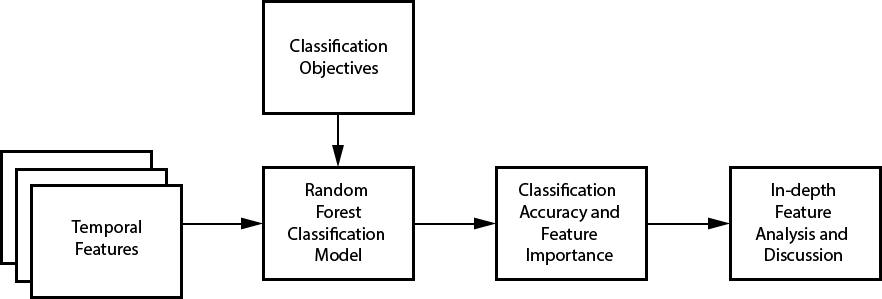
\includegraphics[width=0.98\columnwidth]{figures/characterization_process/characterization_process}
\caption{{Characterization process to investigate the ability for various features to describe the classification objectives
\label{fig:char_process}%
}}
\end{center}
\end{figure}

Random forest classification models were chosen based on their ability to model diverse and large data sets in a robust way \cite{Breiman}. These models use an ensemble of decision trees to predict various characteristic labels about each building based on its features. The literature describes decision trees as the "closest to meeting the requirements for serving as an off-the-shelf procedure for data mining" \cite{hastie_elements_2009}. Figure \ref{fig:decisiontree} illustrates an example of a decision tree using features to determine whether a patient is sick or healthy using two features \cite{Geurts_2009}. 


\begin{figure}[ht!]
\begin{center}
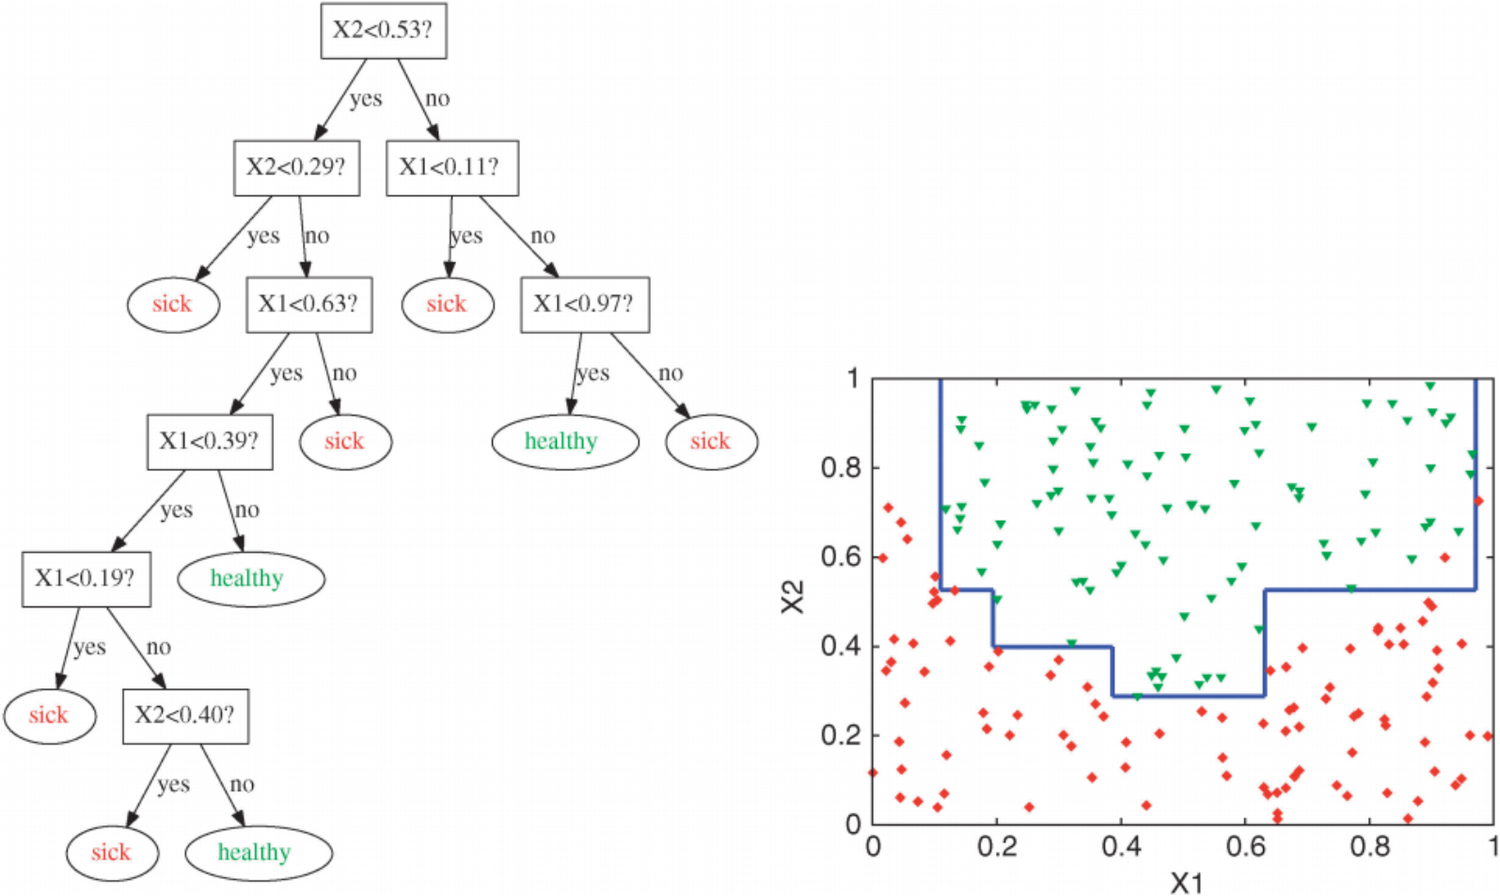
\includegraphics[width=1\columnwidth]{figures/CART_tree_titanic_survivors/decision_tree}
\caption{{An example of a decision tree (left) with the decision boundary for two features, $X1$ and $X2$ (right). Adaption with permission from \cite{Geurts_2009}.
\label{fig:decisiontree}%
}}
\end{center}
\end{figure}

Decision trees often over-fit data due to high variance. Random forest models work by creating a set of decision trees and averaging all of their predictions to overcome this variance. Figure \ref{fig:tree_ensemble} illustrates a set of four decision trees that is more accurately able to distinguish between the two classes than a single tree model.

\begin{figure}[ht!]
\begin{center}
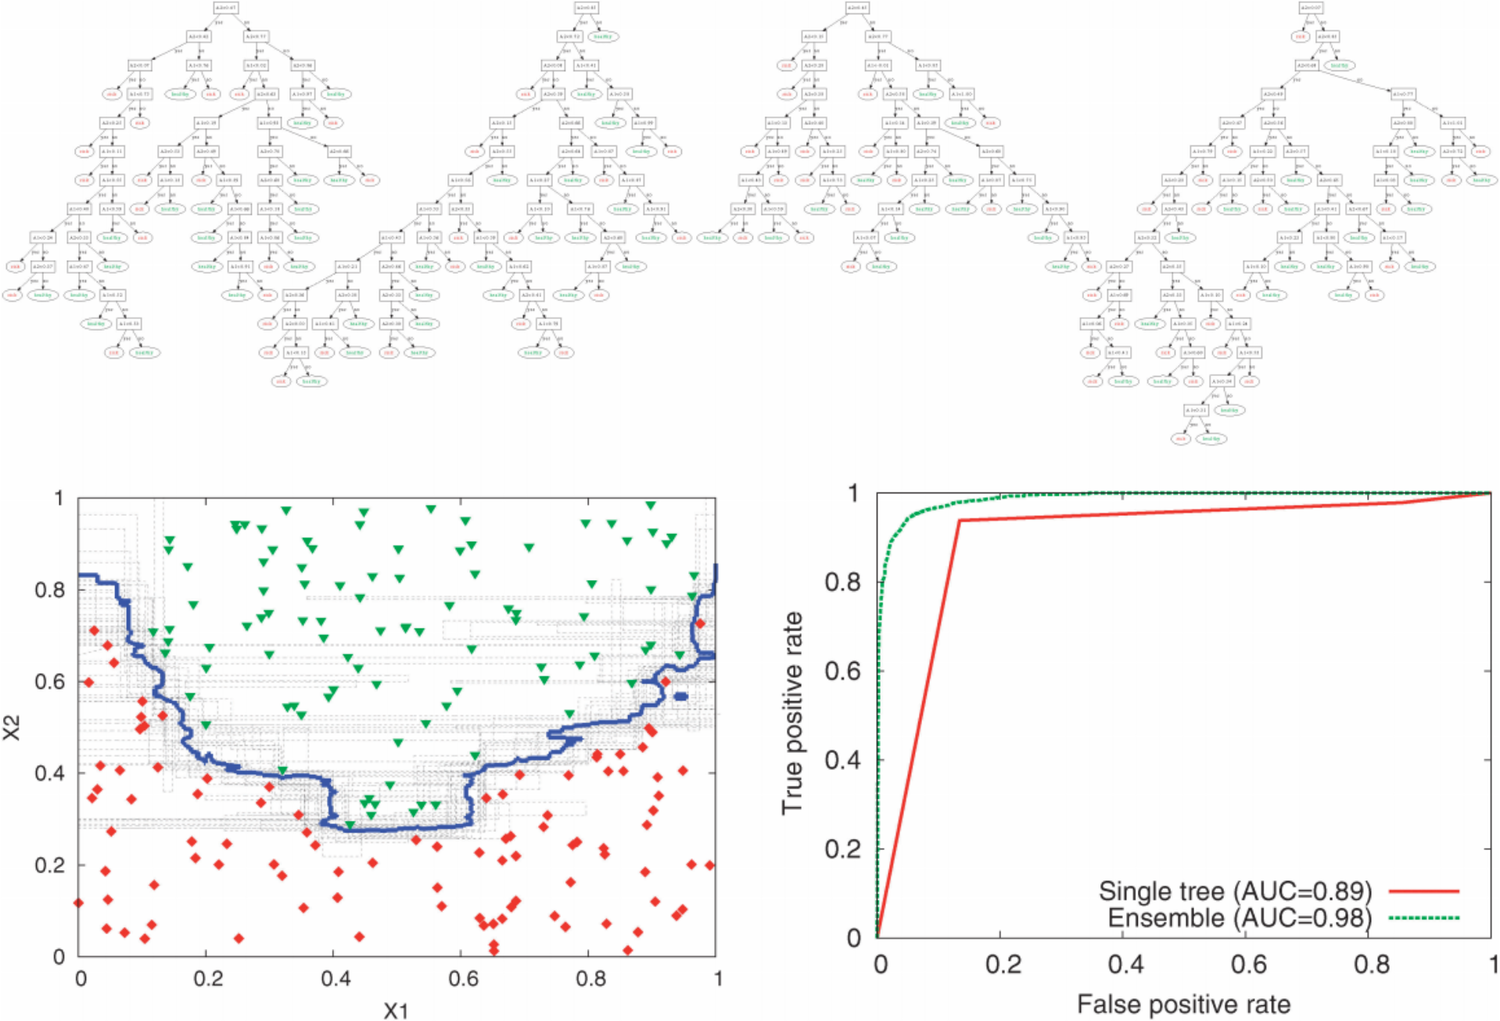
\includegraphics[width=1\columnwidth]{figures/regressiontrees/regressiontrees}
\caption{{Ensemble of decision trees (top) that produces a more accurate decision boundary (lower left) and comparison with a single tree model (lower right). Adapted with permission from \cite{Geurts_2009}.
\label{fig:tree_ensemble}%
}}
\end{center}
\end{figure}

Random forests use a form of cross-validation by training and testing each tree using a different bootstrapped sample from the data. This process produces an \emph{out-of-bag error (OOB)} that acts as a generalized error for understanding how well each class can be predicted. This accuracy is used to determine how well the generated temporal features can delineate the class objectives. Random forests can also calculate the importance of the input features and how well they lend themselves to predicting the objectives. This attribute is useful in that it allows us to understand exactly which temporal features are most characteristic of various objectives. Variable importance is calculated using Equation \ref{eq:varimportance}. The importance of input feature $X_m$ for predicting $Y$ by adding up the weighted impurity decreases $p(t)\Delta i(s_t,t)$ for all nodes $t$ where $X_m$ is used, averaged over all $N_T$ trees in the forest \cite{louppe2013understanding}.

\begin{equation}
Imp(X_m) = \frac{1}{N_T}\sum\limits_T\sum\limits_{t\in T:v(s_t)=X_m} p(t) \Delta i (s_t, t)
\label{eq:varimportance}
\end{equation}

\section{Case Study, Empirical Data Collection, and Qualitative Research}
\label{sec:screeningdata}

% One emerging trend is that "data mining algorithms should have as few parameters as possible, ideally none. A parameter-free algorithm prevents us from imposing our prejudices and presumptions on the problem at hand and let the data itself speak to us \citep{Keogh_2004}." This approach is known as \emph{parameter-free} or \emph{parameter-light} data mining. The efficacy of these algorithms has been proven comparable or better than many more complex, traditional time-series data mining approaches \citep{Keogh_2004}. This mantra is a primary objective of the feature extraction process outlined in this study.

One of the main goals of this research is the testing and implementation of the temporal feature extraction techniques on empirical sensor data collected from real buildings. Various raw data sets were obtained from case study buildings and campuses around the world to test the developed methods. The target of these interactions was to collect at least one year of hourly data from whole building electrical meters, resulting in at least 8760 measurements per building. Several of these data sets were collected through a series of site visits and interviews. These interactions are detailed in Section \ref{sec:sitevisit} by giving an in-depth overview of these case studies by discussing the current performance data acquisition systems and the standard methods of utilizing those data for every day tracking activities. A key goal of the collection of these data was that they would be a basis for an open, shareable data repository for building performance research. This goal was discussed with the case study participants. Several other raw data sets were collected from open data sources on the Internet and were included in this study, albeit often with less metadata available. These case studies are described in Section \ref{openonlinecasestudies}. 

In addition to the quantitative data collected from each of these case studies, qualitative feedback was gathered to get a better sense of \emph{how useful} the implementation and interpretation of the framework would be in the day-to-day operations of various types of stakeholders. The results of these qualitative interviews are included in this Section \ref{sec:characterization}.

\subsection{Site Visits for Case Studies}
\label{sec:sitevisit}
Throughout the course of two years, from February 2014 to April 2016, several site visits were conducted to interview operations staff at seven campuses. The purpose of this effort was two-fold: first, to collect as much raw, temporal data from each site as possible and, second, to discuss the status quo of building energy analysis as performed on their campus. This section discusses these site visits, the types of data that were collected, and a few of the lessons-learned from the process. A consistent theme in the site visits was that each campus has been investing in electrical metering and data acquisition systems over the past decade. In every one of the case study interviews, the operations staff discussed the underutilization of the data being collected. A common phrase was, "We have more meter data than any time before, and we don't know what to do with it." Another common situation was that a campus had a large electrical metering infrastructure but did not know how to extract raw data for this research project. This scenario occurred on three of the seven campuses after the first interview, and data was still not available even after a follow-up visit on two of those campuses. Therefore, only four of the seven case studies had data available and will be discussed in the following subsections.
%The methodology followed in this effort was drawn from mixed-method research techniques.

\subsubsection{Case Study 1} 
\label{sec:casestudy1}
The first case study is a campus in a continental climate in the Midwest region of the United States. It is a university with 226 buildings spread across two main campuses. Altogether, these buildings have a total floor area over 2.3 million square meters (25 million square feet). An initial interview was conducted with the lead statistician of the facilities management in March 2015. Information was gathered on the building and energy management systems of the campus and a discussion regarding the typical utilization of the data was conducted. It was found that there are over 480 electrical meters on the campus and that these data were primarily used for billing of the individual academic departments. They have a custom metering data management platform with some capabilities for data export. A second site visit was conducted in June 2015 to facilitate the collection of a sample one year data set. In this site visit, a facilities management professional with experience in SQL databases was able to directly query the underlying back-end of the energy management system to extract one year of raw data from all of the metering infrastructure on the campus. An accompanying meta-data spreadsheet was discovered that included information on floor area, primary space usage, EnergyStar score, and address. These data were then used for the analysis and feature extraction, and some of the results were compiled and presented to the entire facilities management department of this university in March 2016. This presentation gave an overview of the feature creation techniques and an understanding of how the buildings on their campus compare to other universities. More discussion on the feedback from this presentation are discussed in Section \ref{sec:characterization}.

\subsubsection{Case Study 2}
\label{casestudy2}
The second case study is a campus in the Northeast region of the United States. It is also a University and it has 180 buildings on a single main campus. An initial meeting was organized in April 2015 with the facilities management team. This campus has well-organized building and energy management systems with a strong emphasis on data acquisition and management. The campus has an analytics and automated fault detection software platform that is connected to the underlying controls systems. A follow-up campus visit was conducted in August 2015 to facilitate the download of a raw, example data set from the buildings on campus. At this point, a log-in to a new data management platform was given for the purposes data extraction. Several issues arose from the use of this platform and ultimately, a database query by the software developers of the system was used to extract the one year of electrical meter data from the campus buildings. Once again, a spreadsheet of meta-data was shared that included information on floor area and primary building use type. A final site visit was conducted in April 2016 to discuss some of the results of the data acquisition and upcoming plans for upgrades. A formal presentation of the results was not able to be given; thus only limited feedback of the implementation progress was collected.

\subsubsection{Case Study 3}
\label{sec:casestudy3}

The third case study is a campus in the Midwest region of the United States. Once again, it is a university campus with 25 buildings encompassing 204,000 square meters (2.2 million square feet) of floor space. An initial site survey and discussion of the campus was conducted in March 2015 with the campus lead mechanical and energy engineers. This campus has its electrical meters connected to a campus energy management platform that includes various visualizations and analytics techniques. This platform also can easily provide raw data download for analysis in this study. This platform resulted in this campus being by far the most user-friendly on data collection out of the case study set, including the open, on-line data sources. Raw data in flat files was easily downloaded for all data points at once. The meta-data for this campus was also extracted from this energy management platform, albeit in a more manual method from the user interface. A follow-up visit to this campus was conducted in March 2016 with initial results of characterizing the data according to a subset of the tested features. A significant amount of feedback for this case study was given by the facilities management department regarding the ability for these insights to assist in their decision-making processes. 

\subsubsection{Case Study 4}
\label{sec:casestudy4}

The fourth case study is an international school campus in tropical Southeast Asia. This campus includes five buildings with approximately 58,000 square meters (625,000 square feet). It was built and opened in 2010 and includes some sustainable design features such as an optimized chilled water plant, solar thermal cooling system, and an innovative, fresh air delivery system. The building management and data acquisition system have been a primary focus of the operations director of the campus for many years. Discussions and interviews with the operations staff have occurred numerous times over the course of the last five years. The key focus for this campus has been maintaining an optimized chilled water system. The operations team of this organization has been an active contributor to the development of the methodology. 

\subsubsection{Case Study 5}
\label{sec:casestudy5}

The final case study to be outlined in this section is a university campus located in Switzerland. This campus includes 22 building encompassing more than 150,000 square meters (1.6 million square feet). This campus has an energy management system with the ability to extract raw data, albeit only one point at a time. Data from this campus was utilized in a previous research project focused on campus and building-scale co-simulation and modeling. Only email correspondence with the campus facilities managers of this campus was conducted. A significant amount of meta-data was available from the facilities department through a spreadsheet that provided the breakdown of primary uses of the spaces in each building.

\subsection{Online Open Case Studies}
\label{openonlinecasestudies}

Several large data sets were found through a search of openly accessible data on-line. This section gives an overview of these data sources and the methods in which the data was extracted and pre-processed for analysis. Table \ref{tab:opendata} illustrates these sources, a short description of the platform in which the data was downloaded, and the URL of the platform. As in the site visit case studies, one year of hourly whole building electrical meter data was collected from each of these sources for as many buildings as possible.


\begin{table} 
\label{tab:opendata}
    \begin{tabular}{| p{4cm} | p{4cm} | p{6cm} |}
        \textbf{Source Name} & \textbf{Description} & \textbf{Website}\\
        \hline
        Cornell University & EMCS Portal & http://portal.emcs.cornell.edu/ \\ 
        \hline
        University of California - Berkeley & Berkeley Campus Energy Portal & http://berkeley.openbms.org/\\ 
        \hline
        Arizone State University & Campus Metabolism & https://cm.asu.edu \\ 
        \hline
        Carbon Culture & Community Open Data Platform & https://platform.carbonculture.net \\ 
        \hline
        EnerNOC & EnerNOC GreenButton Data & https://open-enernoc-data.s3.amazonaws.com/anon/ index.html \\         
        \hline
        University of Southamption & Open Data Service & http://data.southampton.ac.uk/\\         
        \hline
    \end{tabular} 
    \caption{Open, online data sources} 
\end{table}


\section{Overview of Data Collected}
\label{sec:datacollected}

Through data collection from the on-site case study interviews and on-line data sources, whole building electrical meter data from 1238 buildings was collected. Figure \ref{fig:casestudymap} illustrates the locations of these building around the world. A majority of the buildings are located in the United States, with the highest concentrations in the northeast region. A wide range of building types are included in the data set, from Education and Government to Agriculture and Heavy Industry. 


\begin{figure}[ht!]
\begin{center}
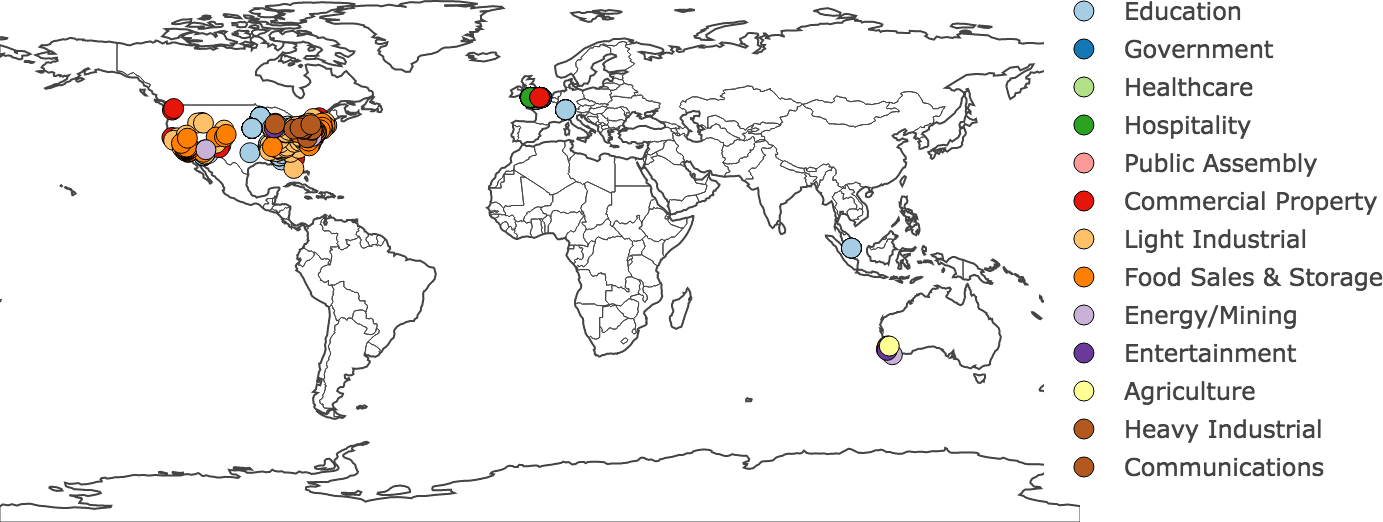
\includegraphics[width=0.98\columnwidth]{figures/casestudybuildinglocations/casestudybuildinglocations}
\caption{Locations of 1238 case study buildings collected from across the world
\label{fig:casestudymap}%
}
\end{center}
\end{figure}

From these groups of primary use types, the buildings are distributed across various time zone regions as seen in Figure \ref{fig:bar_primaryspaceuse}. The east coast of the United States is the largest group due to the number of campuses and buildings from the EnerNOC data source. All of the buildings from the Carbon Culture data source are located in the United Kingdom.

\begin{figure}[ht!]
\begin{center}
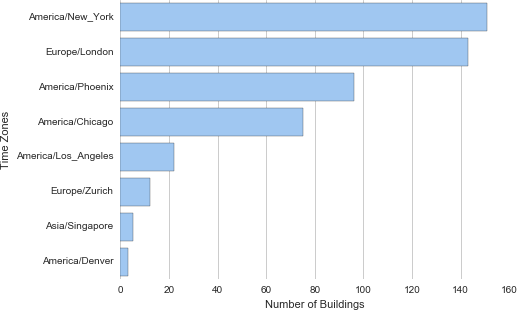
\includegraphics[width=0.98\columnwidth]{figures/timezonesbar1/timezonesbar}
\caption{Distribution of case study buildings amongst time zones
\label{fig:bar_timezone}%
}
\end{center}
\end{figure}

Figure \ref{fig:bar_industry} and \ref{fig:bar_subindustry} illustrate the industries and sub-industries that the case study buildings are collected from. The number of university campuses is strongly evident in both charts.

\begin{figure}[ht!]
\begin{center}
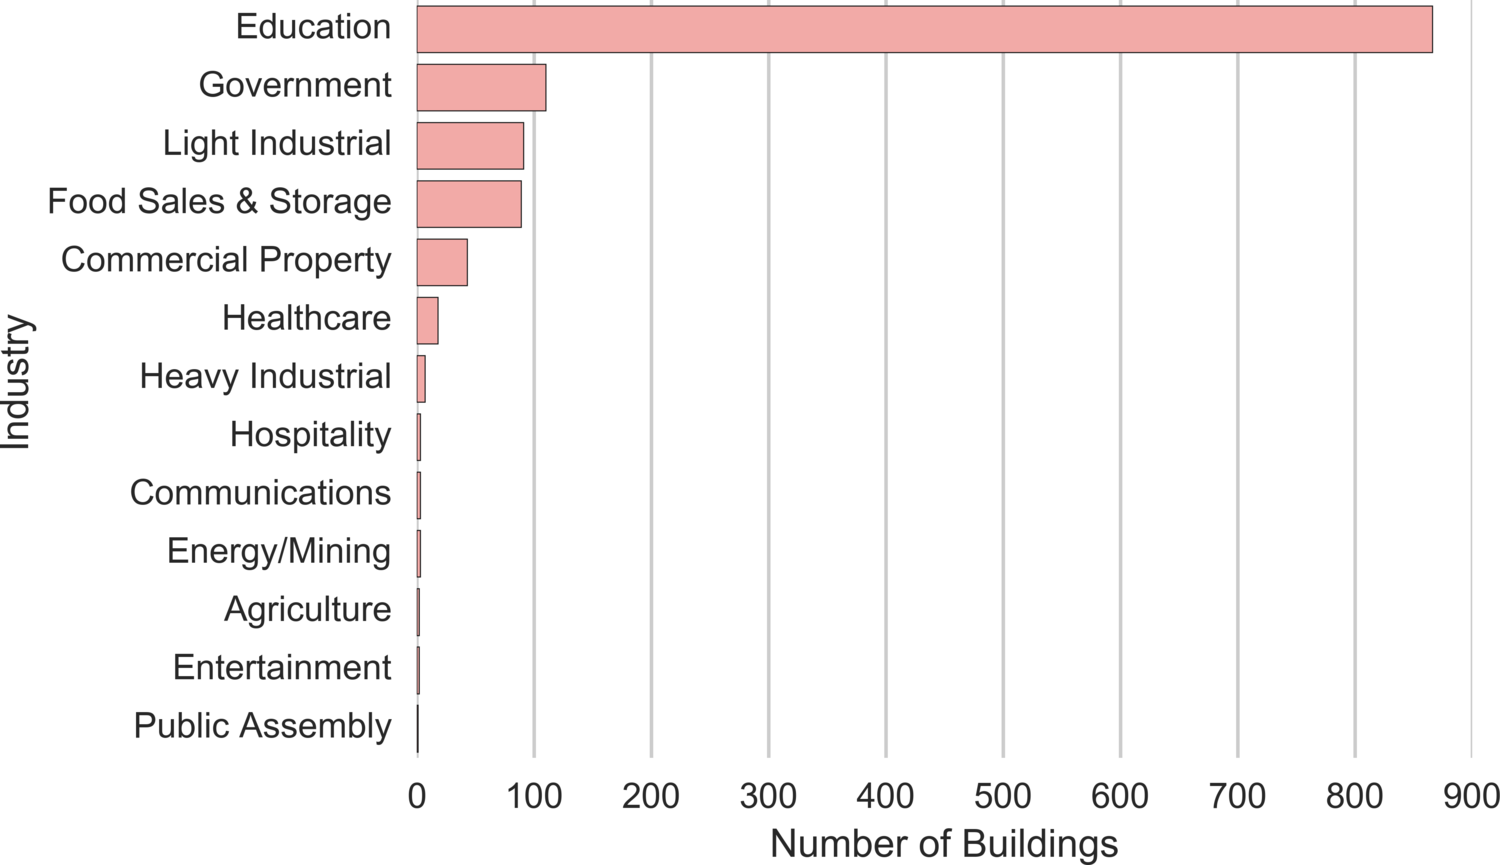
\includegraphics[width=0.98\columnwidth]{figures/bar_industry/bar_industry}
\caption{Distribution of case study buildings amongst general industries
\label{fig:bar_industry}%
}
\end{center}
\end{figure}

\begin{figure}[ht!]
\begin{center}
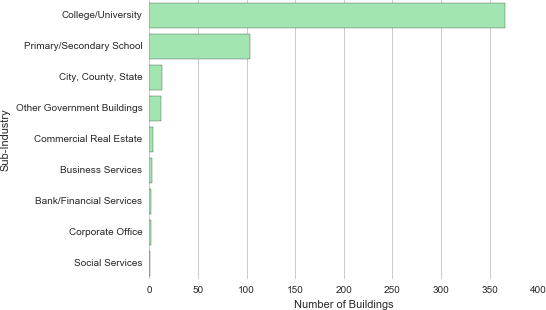
\includegraphics[width=0.98\columnwidth]{figures/bar_subindustry/bar_subindustry}
\caption{Distribution of case study buildings amongst sub-industries
\label{fig:bar_subindustry}%
}
\end{center}
\end{figure}

\subsection{Selection of Case Study Subset for Feature Implementation}
\label{casestudysubset}

A subset of buildings was chosen based on limiting criteria for inclusion in the implementation sections of this thesis. The primary consideration for inclusion is that the building is a member of one of the top primary use types: Offices, Primary/Secondary Schools, University Laboratories, University Classrooms, or Dormitories. These categories and the number of buildings in one are shown in Figure \ref{fig:bar_primaryspaceuse}.

\begin{figure}[ht!]
\begin{center}
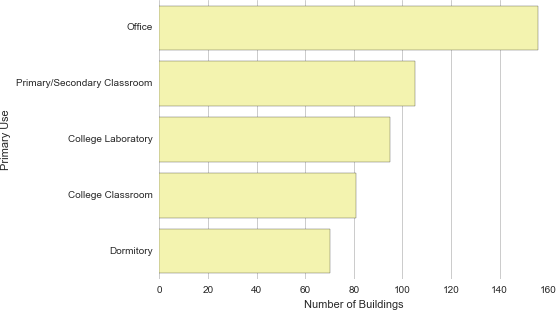
\includegraphics[width=0.98\columnwidth]{figures/bar_primaryspaceuse1/bar_primaryspaceuse}
\caption{Distribution of case study buildings amongst primary space uses
\label{fig:bar_primaryspaceuse}%
}
\end{center}
\end{figure}

\section{Advanced Metering Infrastructure Case Study}
\label{sec:smartmeterdata}

A larger data set of almost 10,000 non-residential buildings is gathered in this thesis from an organization tasked with using the data to target buildings for performance improvement measures. These data are from an Advanced Metering Infrastructure (AMI) implementation. Different types of meta-data are available for these buildings, including industry and energy savings measure implementation. The primary goal of this data set is to provide a context of scalability on a larger data set. These data are strictly private and detailed data cannot be included in the methodology or development of the framework.

